\documentclass[aspectratio=169,14pt]{beamer}
\usetheme{default}
\usepackage{fontspec}
\setmainfont{texgyrepagella-regular.otf}[BoldFont=texgyrepagella-bold.otf,ItalicFont=texgyrepagella-italic.otf,BoldItalicFont=texgyrepagella-bolditalic.otf]
\setsansfont{texgyreheros-regular.otf}[BoldFont=texgyreheros-bold.otf,ItalicFont=texgyreheros-italic.otf,BoldItalicFont=texgyreheros-bold.otf,BoldItalicFeatures={FakeSlant=0.2}]
\setmonofont{lmmono10-regular.otf}[Scale=0.85]
\setbeamertemplate{navigation symbols}{}
\usepackage{pgfpages}
\newif\ifpresenter
\ifdefined\PresenterVersion\presentertrue\else\presenterfalse\fi
\ifpresenter
  \setbeameroption{show notes on second screen=right}
  \setbeamertemplate{note page}[plain]
\fi
\usepackage{amsmath,amssymb,bm,booktabs,array,graphicx,xcolor}
\usepackage{tikz,pgfplots,adjustbox,listings,xurl}
\pgfplotsset{compat=1.18}
\usetikzlibrary{arrows.meta,positioning,calc,fit,shapes.geometric,decorations.pathreplacing,patterns}
% UIUC official brand colors, verified 2026-10-23.
% https://brand.illinois.edu/visual-identity/color
\definecolor{IlliniOrange}{HTML}{FF5F05}
\definecolor{IlliniBlue}{HTML}{13294B}
\definecolor{Storm}{HTML}{707372}
\definecolor{LightStorm}{HTML}{C6C7C6}
\definecolor{Industrial}{HTML}{1D58A7}
\definecolor{Patina}{HTML}{007E8E}
\tikzset{>=Stealth, every node/.style={font=\small,text=IlliniBlue}, box/.style={draw=IlliniBlue,rounded corners=2pt,align=center,inner sep=6pt,execute at begin node=\hyphenpenalty10000\relax}, orangebox/.style={box,draw=IlliniOrange,very thick}, edge/.style={->,thick,IlliniBlue}, accent/.style={->,very thick,IlliniOrange}}
\pgfplotsset{every axis/.append style={width=13.5cm,height=6.5cm,axis line style={IlliniBlue},tick label style={font=\small,text=IlliniBlue},label style={font=\small,text=IlliniBlue},legend style={font=\small,draw=none,fill=white},grid style={LightStorm},major grid style={LightStorm},axis lines=left,clip=false}, every axis plot/.append style={thick}}

\definecolor{slidepaper}{RGB}{234,220,201}
\setbeamercolor{background canvas}{bg=slidepaper}
\setbeamercolor{normal text}{fg=IlliniBlue}
\setbeamercolor{frametitle}{fg=IlliniBlue}
\setbeamercolor{title}{fg=IlliniBlue}
\setbeamercolor{item}{fg=IlliniOrange}
\setbeamerfont{frametitle}{size=\large,series=\bfseries}
\setbeamerfont{title}{size=\Large,series=\bfseries}
\setbeamertemplate{itemize item}{\color{IlliniOrange}$\bullet$}
\setbeamertemplate{itemize subitem}{\color{IlliniOrange}\footnotesize$\circ$}
\setbeamercolor{orangerule}{bg=IlliniOrange}
\setbeamertemplate{headline}{\begin{beamercolorbox}[wd=\paperwidth,ht=0.1cm,dp=0.1cm]{orangerule}\end{beamercolorbox}}
\setbeamertemplate{footline}{\begin{beamercolorbox}[wd=\paperwidth,ht=0.1cm,dp=0.1cm]{orangerule}\end{beamercolorbox}}
\setbeamersize{text margin left=0.65cm,text margin right=0.65cm}
\setlength{\leftmargini}{1.1em}
\newenvironment{slidebullets}{\begin{itemize}\setlength\itemsep{0.8em}}{\end{itemize}}
\pgfplotsset{every axis/.append style={legend style={fill=slidepaper}}}
\lstdefinelanguage{CoursePython}{keywords={from,import,for,in,if,else,def,return,assert,True,False,None},sensitive=true,morecomment=[l]{\#},morestring=[b]',morestring=[b]"}
\lstset{language=CoursePython,basicstyle=\ttfamily\small,keywordstyle=\color{IlliniBlue}\bfseries,commentstyle=\color{Storm},stringstyle=\color{IlliniBlue},showstringspaces=false,breaklines=true,columns=fullflexible,keepspaces=true,frame=none,aboveskip=0.7em,belowskip=0.7em}
\newcommand{\E}{\mathbb E}
\newcommand{\Var}{\operatorname{Var}}
\newcommand{\Cov}{\operatorname{Cov}}
\hypersetup{colorlinks=true,urlcolor=IlliniBlue,linkcolor=IlliniBlue}

\title{Marketing Analytics}
\subtitle{Marketing Decisions and AI-Assisted Coding}
\author{By Nathan Yang}
\date{Session 01}
\begin{document}
\begin{frame}
\titlepage
\end{frame}
\begin{frame}[plain]
\begin{tikzpicture}[remember picture,overlay]
\node[inner sep=0pt] at (current page.center) {
\includegraphics[width=\paperwidth,height=\paperheight,keepaspectratio]{assets/decision_river.png}};
\end{tikzpicture}
\note{A useful analysis connects the available evidence to a feasible decision. Different markets can require different products, margins, and forecasts.

Original conceptual illustration. 05\_Slides/assets/PROVENANCE.md.}
\end{frame}
\begin{frame}{A Renewal Offer}
\usebeamercolor[fg]{normal text}
\vfill
\begin{slidebullets}
\item A subscription firm can contact 5,000 eligible customers.
\item The decision concerns incremental contribution over the next 30 days.
\item Past spending, consent, and account history are available before contact.
\end{slidebullets}
\vfill
\note{The contact budget constrains the action. A high predicted renewal rate can reflect customers who would renew without an offer. The target must include the additional contribution caused by contact.

M1, Section 1.1, Marketing Analytics Lecture Notes. \url{../06_Lecture_Notes/modules/M01_Marketing_Analytics_and_Python.md}}
\end{frame}
\begin{frame}{Analytical Questions}
\usebeamercolor[fg]{normal text}
\vfill
\begin{slidebullets}
\item Description: how often do customers renew?
\item Prediction: who is likely to renew?
\item Causal effect: how does an offer change renewal?
\item Decision: which contacts generate positive incremental contribution?
\end{slidebullets}
\vfill
\note{The same customer records can support different analytical objects. Predictive performance evaluates forecasts under the represented conditions. A targeting policy also needs the untreated comparison and relevant costs.

M1, Section 1.1, Marketing Analytics Lecture Notes. \url{../06_Lecture_Notes/modules/M01_Marketing_Analytics_and_Python.md}}
\end{frame}
\begin{frame}{Incremental Contribution}
\usebeamercolor[fg]{normal text}
\noindent For account $i$, compare renewal under an offer and no offer.
\medskip
\[
\Delta\pi_i=m_i\{p_i(1)-p_i(0)\}-c_i
\]
\medskip
\noindent Contribution $m_i$ and contact cost $c_i$ are dollars per account over the stated horizon.
\note{The formula assumes that the offer cost can be summarized by c and that contribution already deducts relevant variable costs. A discount paid on every treated purchase requires an additional cost term.

M1, Section 1.1, Marketing Analytics Lecture Notes. \url{../06_Lecture_Notes/modules/M01_Marketing_Analytics_and_Python.md}}
\end{frame}
\begin{frame}{Response and Incremental Value}
\usebeamercolor[fg]{normal text}
\centering
\begingroup
\begin{adjustbox}{max width=0.98\textwidth,max totalheight=0.65\textheight}
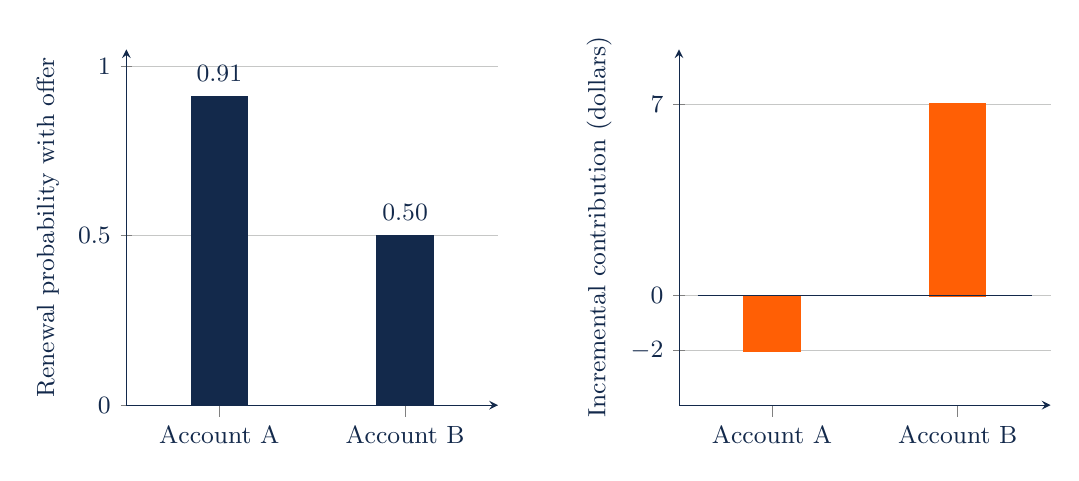
\begin{tikzpicture}
\begin{axis}[name=left,width=6.3cm,height=6.1cm,xmin=.5,xmax=2.5,ybar,bar width=20pt,ymin=0,ymax=1.05,xtick={1,2},xticklabels={Account A,Account B},ylabel={Renewal probability with offer},ytick={0,0.5,1},xmajorgrids=false,ymajorgrids=true]
\addplot[fill=IlliniBlue,draw=IlliniBlue] coordinates {(1,0.91)(2,0.50)};
\node at (axis cs:1,.98) {0.91};\node at (axis cs:2,.57) {0.50};
\end{axis}
\begin{axis}[at={(left.east)},anchor=west,xshift=2.3cm,width=6.3cm,height=6.1cm,xmin=.5,xmax=2.5,ybar,bar width=20pt,ymin=-4,ymax=9,xtick={1,2},xticklabels={Account A,Account B},ylabel={Incremental contribution (dollars)},ytick={-2,0,7},ymajorgrids=true]
\addplot[fill=IlliniOrange,draw=IlliniOrange] coordinates {(1,-2)(2,7)};
\draw[IlliniBlue] (axis cs:.6,0)--(axis cs:2.4,0);
\end{axis}
\end{tikzpicture}

\end{adjustbox}
\endgroup
\par\medskip
{\small Synthetic accounts. Contribution is 100 dollars and contact cost is 3 dollars.\par}
\note{A rises from 0.90 to 0.91. B rises from 0.40 to 0.50. The untreated probabilities explain the reversal. These probabilities are imposed teaching inputs.

M1, Section 1.1, Marketing Analytics Lecture Notes. \url{../06_Lecture_Notes/modules/M01_Marketing_Analytics_and_Python.md}}
\end{frame}
\begin{frame}{The Observation Unit}
\usebeamercolor[fg]{normal text}
\vfill
\begin{slidebullets}
\item A product line, order, customer, and customer-month are different units.
\item The key identifies one row at the intended level.
\item Aggregation changes the weights used in an average.
\end{slidebullets}
\vfill
\note{A customer with five order lines receives five times the weight of a customer with one line in a line-level mean. Define whether the managerial comparison concerns orders or equally weighted customers.

M1, Section 1.2, Marketing Analytics Lecture Notes. \url{../06_Lecture_Notes/modules/M01_Marketing_Analytics_and_Python.md}}
\end{frame}
\begin{frame}[fragile]{Python Objects and Order Totals}
\usebeamercolor[fg]{normal text}
\noindent Three synthetic product lines belong to two orders.
\begin{lstlisting}
lines = [('A', 2, 10), ('A', 1, 5), ('B', 1, 12)]
orders = {}
for order, quantity, price in lines:
    orders[order] = orders.get(order, 0) + quantity * price
total = sum(orders.values())
aov = total / len(orders)
assert (total, aov) == (37, 18.5)
\end{lstlisting}
{\small Check: total sales are 37 dollars and average order value is 18.50 dollars.\par}
\note{The tuple stores an order ID, a quantity, and a unit price. The dictionary accumulates sales by order. The denominator is two orders. Dividing by the three lines gives average line sales.

M1, Section 1.3, Marketing Analytics Lecture Notes. \url{../06_Lecture_Notes/modules/M01_Marketing_Analytics_and_Python.md}}
\end{frame}
\begin{frame}{Functions and Data Contracts}
\usebeamercolor[fg]{normal text}
\vfill
\begin{slidebullets}
\item Inputs have names, types, units, and allowed missing values.
\item A function returns a defined output and an exception report.
\item Returns, canceled orders, and duplicate lines need explicit rules.
\end{slidebullets}
\vfill
\note{A numeric-looking string requires conversion before arithmetic. A negative quantity may be a legitimate return. A rule should preserve a trace from the original record to its inclusion or exclusion.

M1, Section 1.3, Marketing Analytics Lecture Notes. \url{../06_Lecture_Notes/modules/M01_Marketing_Analytics_and_Python.md}}
\end{frame}
\begin{frame}{A Duplicate Lookup Doubles Sales}
\usebeamercolor[fg]{normal text}
\centering
\begingroup
\fontsize{11}{13.2}\selectfont
\def\small{\fontsize{10}{12}\selectfont}
\def\footnotesize{\fontsize{9}{11}\selectfont}
\def\scriptsize{\fontsize{8}{9.5}\selectfont}
\hyphenpenalty=10000
\begin{adjustbox}{max width=0.98\textwidth,max totalheight=0.65\textheight}
% Original synthetic teaching figure; see corresponding module.
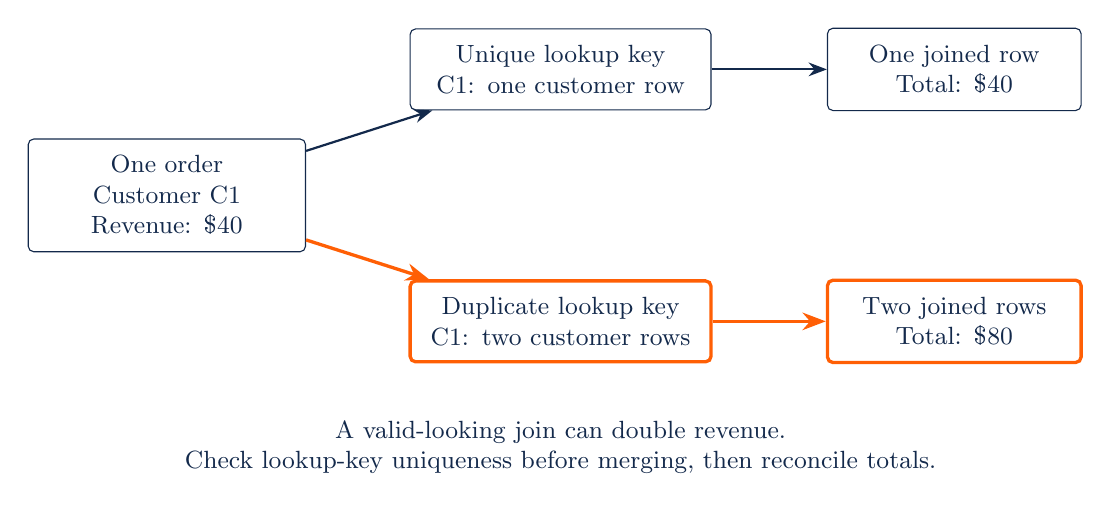
\begin{tikzpicture}
\node[box,text width=3.1cm] (o) at (0,0) {One order\\Customer C1\\Revenue: \$40};
\node[box,text width=3.4cm] (one) at (5,1.6) {Unique lookup key\\C1: one customer row};
\node[orangebox,text width=3.4cm] (two) at (5,-1.6) {Duplicate lookup key\\C1: two customer rows};
\node[box,text width=2.8cm] (good) at (10,1.6) {One joined row\\Total: \$40};
\node[orangebox,text width=2.8cm] (bad) at (10,-1.6) {Two joined rows\\Total: \$80};
\draw[edge] (o)--(one); \draw[accent] (o)--(two);
\draw[edge] (one)--(good); \draw[accent] (two)--(bad);
\node[align=center,text width=11cm] at (5,-3.2) {A valid-looking join can double revenue.\\Check lookup-key uniqueness before merging, then reconcile totals.};
\end{tikzpicture}

\end{adjustbox}
\endgroup
\par\medskip
{\small Synthetic join. One 40-dollar order matches two customer records.\par}
\note{A many-to-one relationship requires unique customer keys in the lookup. Check key uniqueness before merging and reconcile sales afterward.

M1, Section 1.2, Marketing Analytics Lecture Notes. \url{../06_Lecture_Notes/modules/M01_Marketing_Analytics_and_Python.md}}
\end{frame}
\begin{frame}{An AI Coding Request}
\usebeamercolor[fg]{normal text}
\vfill
\begin{slidebullets}
\item Return one row per order and an exceptions table.
\item Treat negative quantities as returns under the stated rule.
\item Verify the 37-dollar example and reject missing order IDs.
\item Explain each transformation before adding the next step.
\end{slidebullets}
\vfill
\note{A useful request specifies analytical behavior and acceptance criteria. The assistant can propose an implementation while the analyst remains responsible for the observation unit and sample rules.

M1, Section 1.5, Marketing Analytics Lecture Notes. \url{../06_Lecture_Notes/modules/M01_Marketing_Analytics_and_Python.md}}
\end{frame}
\begin{frame}{Code Errors and Missing Evidence}
\usebeamercolor[fg]{normal text}
\vfill
\begin{slidebullets}
\item A repeated daily total requires a correction to aggregation.
\item Unrecorded food requires additional measurement or a recorded-behavior target.
\item A coupon decision needs evidence about untreated outcomes.
\end{slidebullets}
\vfill
\note{The response to a failed analysis depends on the unresolved distinction. Ask for the smallest check that could distinguish a calculation error from missing information. A new model can improve implementation while leaving the missing-information problem unchanged. A validated category summary can also remove unnecessary prose generation when the decision only needs category totals.

Marketing Analytics Lecture Notes, M1 §1.12.}
\end{frame}
\begin{frame}{Verification With Counterexamples}
\usebeamercolor[fg]{normal text}
\vfill
\begin{slidebullets}
\item A duplicate lookup must trigger a failed key check.
\item An unmatched customer must remain visible in the assessment.
\item An empty input needs an explicit result.
\item Order totals must reconcile with eligible product lines.
\end{slidebullets}
\vfill
\note{These checks test properties that can fail even when code runs. Repeating the program with the same input confirms reproducibility but does not independently establish correctness.

M1, Section 1.5, Marketing Analytics Lecture Notes. \url{../06_Lecture_Notes/modules/M01_Marketing_Analytics_and_Python.md}}
\end{frame}
\begin{frame}{mHealth Records}
\usebeamercolor[fg]{normal text}
\vfill
\begin{slidebullets}
\item Food entries describe recorded items on observed user-days.
\item The separate daily table covers only part of the food-log history.
\item Reported daily calories repeat across item rows.
\end{slidebullets}
\vfill
\note{The released records replace user identifiers and birthdays and perturb weight values. The source daily total is distinct from the sum of item calories. Neither is a direct measure of complete usual intake.

M1, Section 1.8, Marketing Analytics Lecture Notes. \url{../06_Lecture_Notes/modules/M01_Marketing_Analytics_and_Python.md}}
\end{frame}
\begin{frame}{Join Choice Changes the Sample}
\usebeamercolor[fg]{normal text}
\centering
\begingroup
\fontsize{11}{13.2}\selectfont
\def\small{\fontsize{10}{12}\selectfont}
\def\footnotesize{\fontsize{9}{11}\selectfont}
\def\scriptsize{\fontsize{8}{9.5}\selectfont}
\hyphenpenalty=10000
\begin{adjustbox}{max width=0.98\textwidth,max totalheight=0.65\textheight}
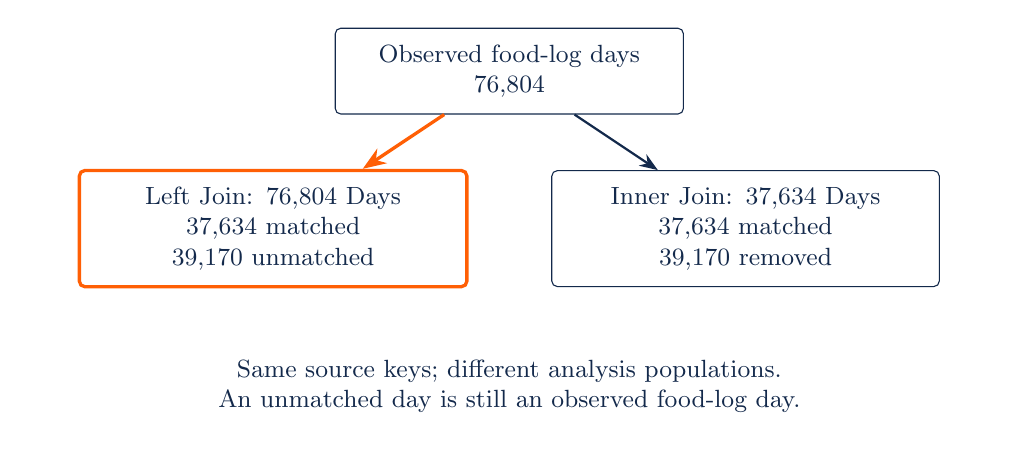
\begin{tikzpicture}
\node[box,text width=4cm] (start) at (0,0) {Observed food-log days\\76,804};
\node[orangebox,text width=4.5cm] (left) at (-3,-2) {Left Join: 76,804 Days\\37,634 matched\\39,170 unmatched};
\node[box,text width=4.5cm] (inner) at (3,-2) {Inner Join: 37,634 Days\\37,634 matched\\39,170 removed};
\draw[accent] (start) -- (left);
\draw[edge] (start) -- (inner);
\node[align=center,text width=12cm] at (0,-4) {Same source keys; different analysis populations.\\An unmatched day is still an observed food-log day.};
\end{tikzpicture}

\end{adjustbox}
\endgroup
\par\medskip
{\small Released mHealth cohort: 76,804 observed user-days.\par}
\note{An inner join would remove more than half the cohort days. Missing calendar days are separate from unmatched rows in a join. The fixed cohort rule preserves within-user histories.

M1, Section 1.8.2, Marketing Analytics Lecture Notes. \url{../06_Lecture_Notes/modules/M01_Marketing_Analytics_and_Python.md}}
\end{frame}
\begin{frame}{Coding Exercise: An Order Assessment}
\usebeamercolor[fg]{normal text}
\vfill
\begin{slidebullets}
\item Implement aggregation with a coding assistant.
\item Add a return, a missing identifier, and a duplicated lookup key.
\item Report how each change affects rows, totals, and exceptions.
\end{slidebullets}
\vfill
\note{Use the small example in ../03\_Data\_and\_Code/Lecture\_Examples/session\_examples.py S01. Retain the original three-line example as a hand-check. The output should distinguish accepted records from records requiring a decision.

M1, Section 1.5, Marketing Analytics Lecture Notes. \url{../06_Lecture_Notes/modules/M01_Marketing_Analytics_and_Python.md}}
\end{frame}
\begin{frame}{Versioned Evidence}
\usebeamercolor[fg]{normal text}
\vfill
\begin{slidebullets}
\item Record the model, date, prompts, tools, settings, parser, and scoring rule.
\item Keep known failure cases and evaluate transfer on fresh cases.
\item Check parsing, execution, and analytical correctness separately.
\end{slidebullets}
\vfill
\note{A historical finding concerns the tested configuration. A current workflow can differ through the model, interface, data, or judgment rule. Chen, Zaharia, and Zou separate code formatting from correctness after postprocessing. A code generator can improve on one measure while an automated pipeline breaks on another.

M1 §1.13. Chen, Zaharia, and Zou (2024), §3.5. \url{https://hdsr.mitpress.mit.edu/pub/y95zitmz/release/2} \url{../01_Resources/14_LLM_Evidence_and_Revalidation/README.md}}
\end{frame}
\begin{frame}{A Reproducible Analysis}
\usebeamercolor[fg]{normal text}
\vfill
\begin{slidebullets}
\item Relative paths identify inputs and outputs.
\item A fresh run reconstructs results without hidden notebook state.
\item Record package versions and consequential AI contributions.
\end{slidebullets}
\vfill
\note{A random seed reproduces a particular random computation under a given implementation. It does not establish valid sampling or eliminate changes across software versions.

M1, Section 1.3, Marketing Analytics Lecture Notes. \url{../06_Lecture_Notes/modules/M01_Marketing_Analytics_and_Python.md}}
\end{frame}
\begin{frame}{A Campaign Specification}
\usebeamercolor[fg]{normal text}
\vfill
\begin{slidebullets}
\item Define the eligible customers and contact date.
\item State the contribution horizon and relevant costs.
\item Identify the evidence needed for the untreated outcome.
\item Choose a numerical check that would reveal a wrong denominator.
\end{slidebullets}
\vfill
\note{The specification should state one feasible action and the comparison that supports it. A randomized pilot may be the next useful step when incremental response is unresolved.

M1, Section 1.4, Marketing Analytics Lecture Notes. \url{../06_Lecture_Notes/modules/M01_Marketing_Analytics_and_Python.md}}
\end{frame}
\begin{frame}{Customer Data in an AI Workflow}
\usebeamercolor[fg]{normal text}
\vfill
\begin{slidebullets}
\item Use only data authorized for the tool and task.
\item Minimize fields and use synthetic examples when they suffice.
\item Check where uploads, logs, and generated files are stored.
\end{slidebullets}
\vfill
\note{Public availability does not establish permission for every reuse. Pseudonymized histories can retain identifying patterns. A coding request should specify the permitted input and destination before any transfer.

Course agent guide and ETHICS\_AND\_REGULATION.md, M1.}
\end{frame}
\begin{frame}{Decision Discussion}
\usebeamercolor[fg]{normal text}
\vfill
\begin{slidebullets}
\item Which customer receives the renewal offer?
\item What changes if every treated renewal receives a discount?
\item Which future variable would invalidate a Monday-morning forecast?
\end{slidebullets}
\vfill
\note{Under the stated synthetic inputs, B has higher incremental contribution. A discount paid to every renewing recipient reduces value by the treated renewal probability times the discount. A Wednesday service contact is unavailable for a Monday forecast.

M1, Section 1.6, Marketing Analytics Lecture Notes. \url{../06_Lecture_Notes/modules/M01_Marketing_Analytics_and_Python.md}}
\end{frame}
\end{document}
